\documentclass[a4paper,draft=false]{scrreprt}\usepackage[]{graphicx}\usepackage[]{color}
%% maxwidth is the original width if it is less than linewidth
%% otherwise use linewidth (to make sure the graphics do not exceed the margin)
\makeatletter
\def\maxwidth{ %
  \ifdim\Gin@nat@width>\linewidth
    \linewidth
  \else
    \Gin@nat@width
  \fi
}
\makeatother

\definecolor{fgcolor}{rgb}{0.345, 0.345, 0.345}
\newcommand{\hlnum}[1]{\textcolor[rgb]{0.686,0.059,0.569}{#1}}%
\newcommand{\hlstr}[1]{\textcolor[rgb]{0.192,0.494,0.8}{#1}}%
\newcommand{\hlcom}[1]{\textcolor[rgb]{0.678,0.584,0.686}{\textit{#1}}}%
\newcommand{\hlopt}[1]{\textcolor[rgb]{0,0,0}{#1}}%
\newcommand{\hlstd}[1]{\textcolor[rgb]{0.345,0.345,0.345}{#1}}%
\newcommand{\hlkwa}[1]{\textcolor[rgb]{0.161,0.373,0.58}{\textbf{#1}}}%
\newcommand{\hlkwb}[1]{\textcolor[rgb]{0.69,0.353,0.396}{#1}}%
\newcommand{\hlkwc}[1]{\textcolor[rgb]{0.333,0.667,0.333}{#1}}%
\newcommand{\hlkwd}[1]{\textcolor[rgb]{0.737,0.353,0.396}{\textbf{#1}}}%

\usepackage{framed}
\makeatletter
\newenvironment{kframe}{%
 \def\at@end@of@kframe{}%
 \ifinner\ifhmode%
  \def\at@end@of@kframe{\end{minipage}}%
  \begin{minipage}{\columnwidth}%
 \fi\fi%
 \def\FrameCommand##1{\hskip\@totalleftmargin \hskip-\fboxsep
 \colorbox{shadecolor}{##1}\hskip-\fboxsep
     % There is no \\@totalrightmargin, so:
     \hskip-\linewidth \hskip-\@totalleftmargin \hskip\columnwidth}%
 \MakeFramed {\advance\hsize-\width
   \@totalleftmargin\z@ \linewidth\hsize
   \@setminipage}}%
 {\par\unskip\endMakeFramed%
 \at@end@of@kframe}
\makeatother

\definecolor{shadecolor}{rgb}{.97, .97, .97}
\definecolor{messagecolor}{rgb}{0, 0, 0}
\definecolor{warningcolor}{rgb}{1, 0, 1}
\definecolor{errorcolor}{rgb}{1, 0, 0}
\newenvironment{knitrout}{}{} % an empty environment to be redefined in TeX

\usepackage{alltt}

\usepackage[utf8]{inputenc}
\usepackage[T1]{fontenc}
\usepackage[english]{babel}

\usepackage{amsmath}
\usepackage{amssymb}

\usepackage{graphicx}

\usepackage{appendix}

\addto{\captionsenglish}{\renewcommand{\bibname}{R and R packages}}

%%%%%%%%%%%%%%%%%%%%%%%%%%%%%%%%%%%%%%%%%%%%%%%%%%
% info to go to titlepage
\subject{Case 1}
\title{Damage detection of the Valdemar platform model}
%\subtitle{subtitle}
\author{Kasper Juul Jensen, Lars Roed Ingerslev, Maya Katrin Gussmann}
%\date{\today}

%%%%%%%%%%%%%%%%%%%%%%%%%%%%%%%%%%%%%%%%%%%%%%%%%%
\IfFileExists{upquote.sty}{\usepackage{upquote}}{}
\begin{document}
% Titlepage
\maketitle

% Rnw options need to be set to knitr, not to Sweave!!
% knitr setup:


Please upload a file \verb+yhat.txt+ containing predictions $\lbrace 0, 1, 2, 3\rbrace$ as one long vector with newline separating the observations. The corresponding order is that given in the \mbox{Cas1\_tst} (Xt), and a small report with a brief introduction/abstract, pre-processing, modeling and model assessment, plus your evaluation of the actual dimensions needed to describe the data/problem. (Max 5	A4 pages of text)

Please note that the deadline is mid-day.

\chapter{Introduction} % Kasper

There are three sensors on an offshore platform, that record data for detecting damage to the platform. Damage can occur at three different sites (see table \ref{table:damageclass}) and for three different intensities ($5\%, 10\%, 15\%$). The recorded data is given in the form of Frequency Response Functions (FRFs).

\begin{table}[ht]
\begin{center}
\begin{tabular}{ll}
  \hline
  Class & Description\\\hline
  0 & undamaged\\
  1 & damage in the bottom of the shaft\\
  2 & damage in one of the legs\\
  3 & damage in the top of the shaft\\
  \hline
\end{tabular}
\caption{Damage classes.\label{table:damageclass}}
\end{center}
\end{table}

In this case, $4092$ samples of the three FRFs for $190$ cases are given, together with their respective damage classes. The goal is to form a model to predict damage and damage class.

\begin{figure}[hb]
\begin{center}
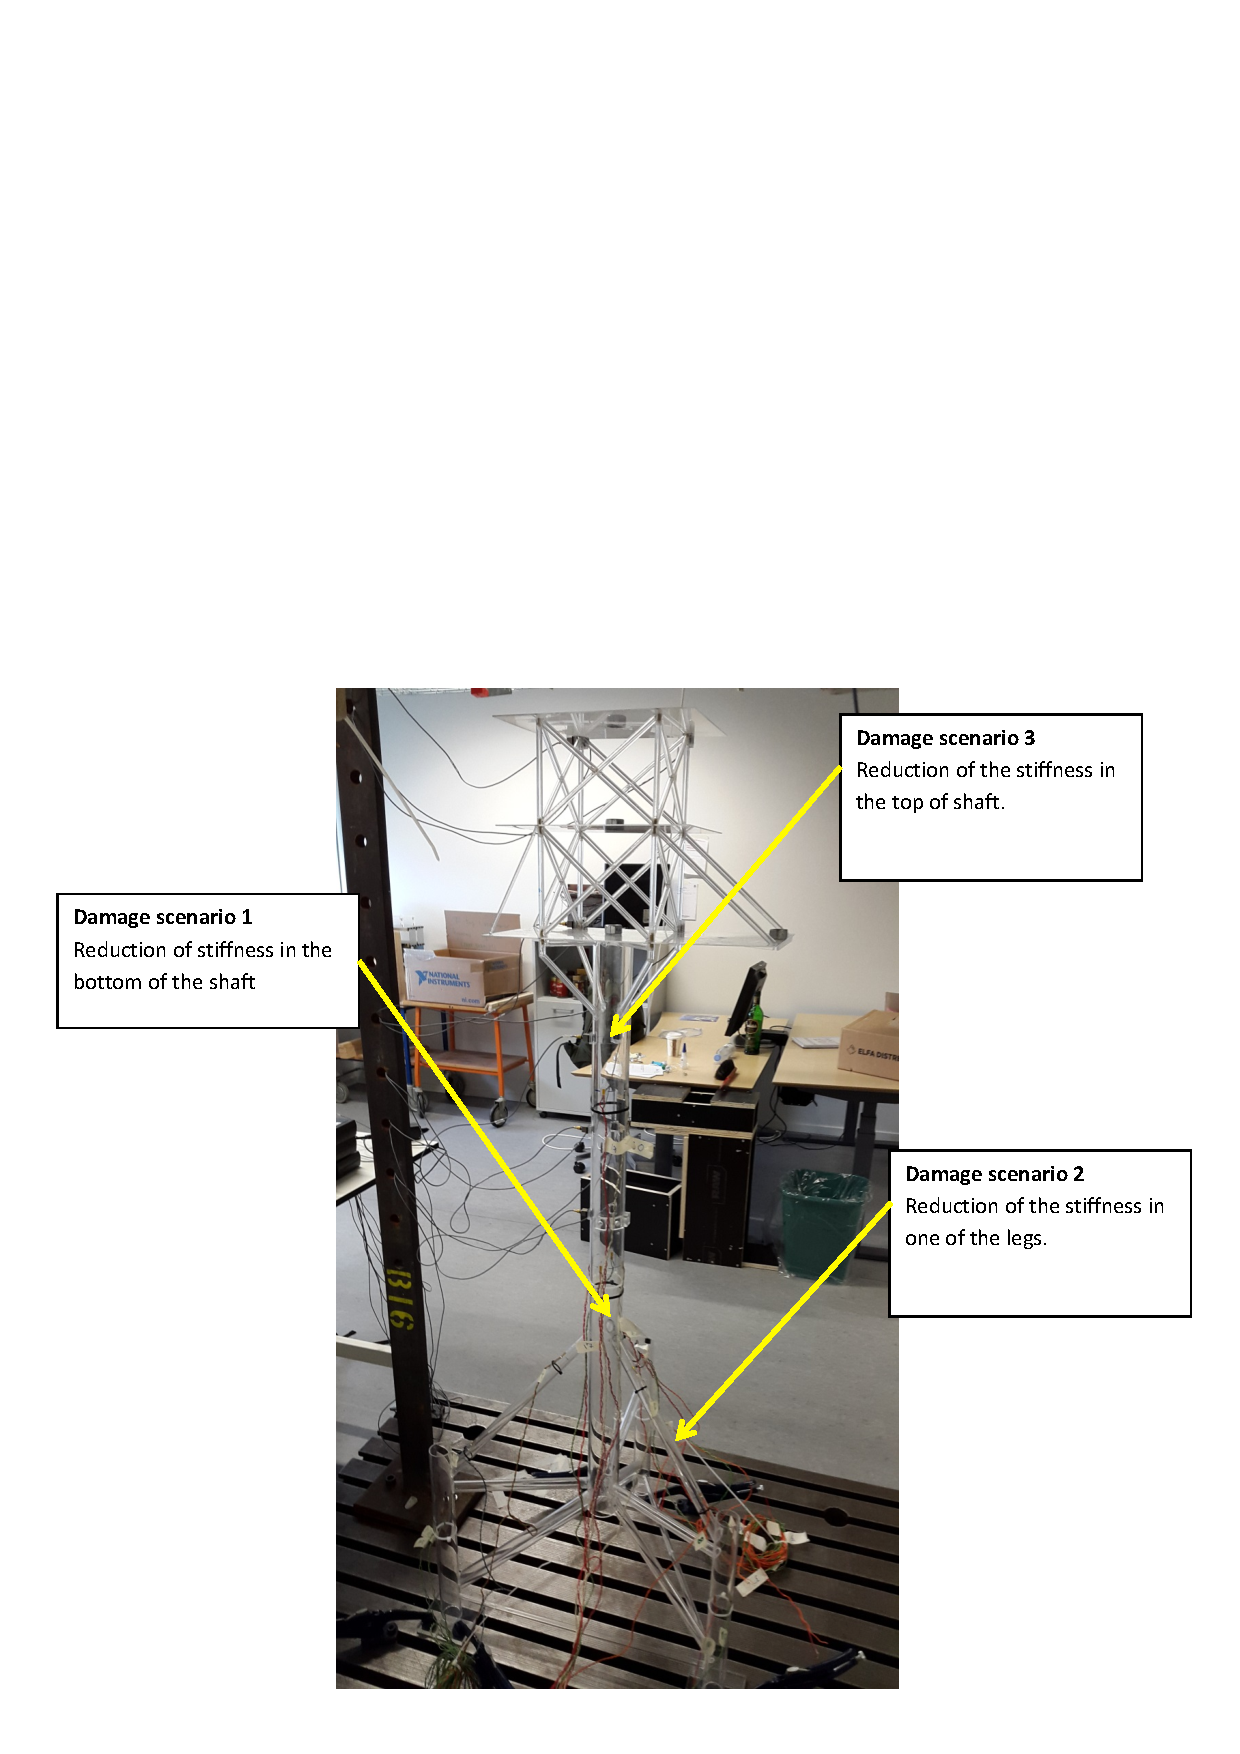
\includegraphics[width=0.6\textwidth]{Valdemarplatform}
\end{center}
\end{figure}

\chapter{Pre-processing}
\section{Cross validation} % Lars
\section{PLS} % Lars

\chapter{Modeling}
% These are not included, but are needed for reference


In the following sections we will look into different models. The final damage class will then be chosen based on a majority vote of the models.

\section{KNN} % Kasper
\begin{knitrout}
\definecolor{shadecolor}{rgb}{0.969, 0.969, 0.969}\color{fgcolor}\begin{kframe}
\begin{alltt}
\hlstd{KNNfn} \hlkwb{<-} \hlkwa{function}\hlstd{(}\hlkwc{xTrain}\hlstd{,} \hlkwc{yTrain}\hlstd{,} \hlkwc{xTest}\hlstd{,} \hlkwc{yTest}\hlstd{,} \hlkwc{nNeighbours}\hlstd{)}
\hlstd{\{}
    \hlstd{errKNNcv} \hlkwb{<-} \hlkwd{numeric}\hlstd{(nNeighbours)}
    \hlcom{# Use leave one out CV of train set to select number of neighbours}
    \hlkwa{for} \hlstd{(K} \hlkwa{in} \hlkwd{seq_len}\hlstd{(nNeighbours))}
    \hlstd{\{}
      \hlstd{KNNpred} \hlkwb{<-} \hlkwd{knn.cv}\hlstd{(}\hlkwc{train} \hlstd{= xTrain,} \hlkwc{cl} \hlstd{= yTrain,} \hlkwc{k} \hlstd{= K)}
      \hlstd{errKNNcv[K]} \hlkwb{<-} \hlkwd{sum}\hlstd{(}\hlkwd{as.integer}\hlstd{(KNNpred} \hlopt{!=} \hlstd{yTrain))}
    \hlstd{\}}
    \hlcom{# The simplest model is the one with the most neighbours}
    \hlstd{K} \hlkwb{<-} \hlkwd{max}\hlstd{(}\hlkwd{which}\hlstd{(errKNNcv} \hlopt{==} \hlkwd{min}\hlstd{(errKNNcv)))}

    \hlstd{KNNpred} \hlkwb{<-} \hlkwd{knn}\hlstd{(}\hlkwc{train} \hlstd{= xTrain,} \hlkwc{test} \hlstd{= xTest,} \hlkwc{cl} \hlstd{= yTrain,} \hlkwc{k} \hlstd{= K)}
    \hlstd{errKNN} \hlkwb{<-} \hlkwd{sum}\hlstd{(}\hlkwd{as.integer}\hlstd{(KNNpred} \hlopt{!=} \hlstd{yTest))}
    \hlkwd{names}\hlstd{(errKNN)} \hlkwb{<-} \hlstr{"KNN"}

    \hlkwd{print}\hlstd{(K)}

    \hlkwd{list}\hlstd{(}\hlkwc{errorRate} \hlstd{= errKNN,} \hlkwc{predictions} \hlstd{= KNNpred)}
\hlstd{\}}
\end{alltt}
\end{kframe}
\end{knitrout}

\section{Logistic regression} % Lars
\begin{knitrout}
\definecolor{shadecolor}{rgb}{0.969, 0.969, 0.969}\color{fgcolor}\begin{kframe}
\begin{alltt}
\hlstd{logisticRegressionFn} \hlkwb{<-} \hlkwa{function}\hlstd{(}\hlkwc{xTrain}\hlstd{,} \hlkwc{yTrain}\hlstd{,} \hlkwc{xTest}\hlstd{,} \hlkwc{yTest}\hlstd{)\{}
    \hlstd{maxVal} \hlkwb{<-} \hlkwd{max}\hlstd{(}\hlkwd{abs}\hlstd{(xTrain))}
    \hlstd{dat} \hlkwb{<-} \hlkwd{data.frame}\hlstd{(}\hlkwc{y} \hlstd{= yTrain,} \hlkwd{unclass}\hlstd{(xTrain}\hlopt{/}\hlstd{maxVal))}
    \hlstd{model} \hlkwb{<-} \hlkwd{multinom}\hlstd{(y} \hlopt{~} \hlstd{.,} \hlkwc{data} \hlstd{= dat)}
    \hlstd{logitPred} \hlkwb{<-} \hlkwd{predict}\hlstd{(model,} \hlkwc{newdata}\hlstd{=} \hlkwd{data.frame}\hlstd{(xTest}\hlopt{/}\hlstd{maxVal),} \hlkwc{type}\hlstd{=}\hlstr{'probs'}\hlstd{)}

    \hlstd{logitPred} \hlkwb{<-} \hlkwd{factor}\hlstd{(}\hlkwd{apply}\hlstd{(logitPred,} \hlnum{1}\hlstd{, which.max)} \hlopt{-} \hlnum{1}\hlstd{,} \hlkwc{levels} \hlstd{=} \hlkwd{c}\hlstd{(}\hlnum{0}\hlopt{:}\hlnum{3}\hlstd{))}
    \hlstd{errLogit} \hlkwb{<-} \hlkwd{sum}\hlstd{(logitPred} \hlopt{!=} \hlstd{yTest)} \hlopt{/} \hlkwd{length}\hlstd{(yTest)}
    \hlkwd{names}\hlstd{(errLogit)} \hlkwb{<-} \hlstr{"LogisticRegression"}

    \hlkwd{list}\hlstd{(}\hlkwc{errorRate} \hlstd{= errLogit,} \hlkwc{predictions} \hlstd{= logitPred)}
\hlstd{\}}
\end{alltt}
\end{kframe}
\end{knitrout}

\section{SVM} % Maya
We used a support vector machine \cite{e1071} with a linear kernel to build a model from the training data. Then, classes for the test data were predicted and the error rate calculated. The mean error rate for this model was $0.00$, see table \ref{table:meanerror}. For the given training and test data and pre-processing, the SVM is performing very well.
\begin{knitrout}
\definecolor{shadecolor}{rgb}{0.969, 0.969, 0.969}\color{fgcolor}\begin{kframe}
\begin{alltt}
\hlstd{svmFn} \hlkwb{<-} \hlkwa{function}\hlstd{(}\hlkwc{xTrain}\hlstd{,} \hlkwc{yTrain}\hlstd{,} \hlkwc{xTest}\hlstd{,} \hlkwc{yTest}\hlstd{)\{}
    \hlstd{dat} \hlkwb{<-} \hlkwd{data.frame}\hlstd{(}\hlkwc{y} \hlstd{= yTrain,} \hlkwd{unclass}\hlstd{(xTrain))}
    \hlkwd{colnames}\hlstd{(dat)} \hlkwb{<-} \hlkwd{c}\hlstd{(}\hlstr{'y'}\hlstd{,} \hlkwd{colnames}\hlstd{(xTrain))}
    \hlstd{model} \hlkwb{<-} \hlkwd{svm}\hlstd{(}\hlkwc{formula} \hlstd{= y} \hlopt{~} \hlstd{.,} \hlkwc{data} \hlstd{= dat,} \hlkwc{kernel} \hlstd{=} \hlstr{"linear"}\hlstd{)}

    \hlstd{svmPred} \hlkwb{<-} \hlkwd{predict}\hlstd{(model, xTest)}
    \hlstd{errSVM} \hlkwb{<-} \hlkwd{sum}\hlstd{(svmPred} \hlopt{!=} \hlstd{yTest)} \hlopt{/} \hlkwd{length}\hlstd{(yTest)}
    \hlkwd{names}\hlstd{(errSVM)} \hlkwb{<-} \hlstr{"SVM"}

    \hlkwd{list}\hlstd{(}\hlkwc{errorRate} \hlstd{= errSVM,} \hlkwc{predictions} \hlstd{= svmPred)}
\hlstd{\}}
\end{alltt}
\end{kframe}
\end{knitrout}

\section{CART} % Maya
For the classification and regression trees we used the \verb+rpart+ function to fit a classification tree and \verb+prune+ to prune it, if necessary, \cite{rpart}. The mean error rate for CART was $0.01$, which is slightly worse than for some of the other models, see table \ref{table:meanerror}.

\begin{knitrout}
\definecolor{shadecolor}{rgb}{0.969, 0.969, 0.969}\color{fgcolor}\begin{kframe}
\begin{alltt}
\hlstd{cartFn} \hlkwb{<-} \hlkwa{function}\hlstd{(}\hlkwc{xTrain}\hlstd{,} \hlkwc{yTrain}\hlstd{,} \hlkwc{xTest}\hlstd{,} \hlkwc{yTest}\hlstd{)}
\hlstd{\{}
    \hlstd{dat} \hlkwb{<-} \hlkwd{data.frame}\hlstd{(}\hlkwc{y} \hlstd{= yTrain,} \hlkwd{unclass}\hlstd{(xTrain))}
    \hlstd{model} \hlkwb{<-} \hlkwd{rpart}\hlstd{(y} \hlopt{~} \hlstd{.,} \hlkwc{data} \hlstd{= dat,} \hlkwc{method} \hlstd{=} \hlstr{"class"}\hlstd{)}
    \hlstd{pfit}\hlkwb{<-} \hlkwd{prune}\hlstd{(model,} \hlkwc{cp}\hlstd{= model}\hlopt{$}\hlstd{cptable[}\hlkwd{which.min}\hlstd{(model}\hlopt{$}\hlstd{cptable[,}\hlstr{"xerror"}\hlstd{]),}\hlstr{"CP"}\hlstd{])}

    \hlstd{cartPred} \hlkwb{<-} \hlkwd{predict}\hlstd{(pfit,} \hlkwc{newdata} \hlstd{=} \hlkwd{data.frame}\hlstd{(xTest),} \hlkwc{type} \hlstd{=} \hlkwd{c}\hlstd{(}\hlstr{"class"}\hlstd{))}
    \hlstd{errCart} \hlkwb{<-} \hlkwd{sum}\hlstd{(cartPred} \hlopt{!=} \hlstd{yTest)} \hlopt{/} \hlkwd{length}\hlstd{(yTest)}
    \hlkwd{names}\hlstd{(errCart)} \hlkwb{<-} \hlstr{"CART"}

    \hlkwd{list}\hlstd{(}\hlkwc{errorRate} \hlstd{= errCart,} \hlkwc{predictions} \hlstd{= cartPred)}
\hlstd{\}}
\end{alltt}
\end{kframe}
\end{knitrout}

\section{Boosting} % Kasper
\section{Random Forest} % Lars
\section{Majority Vote} % 
For the final class selection, we compared all model predictions and chose the class that was predicted by most models. In case of a tie, the first used method (see table \ref{table:meanerror}) would be chosen. For the R-code of the majority vote, please see appendix \ref{appendix:vote}.


% latex table generated in R 3.2.2 by xtable 1.7-4 package
% Mon Mar 21 14:01:37 2016
\begin{table}[ht]
\centering
\begin{tabular}{rr}
  \hline
 & x \\ 
  \hline
KNN & 0.00 \\ 
  LogisticRegression & 0.01 \\ 
  SVM & 0.00 \\ 
  CART & 0.01 \\ 
  majorityVote & 0.00 \\ 
   \hline
\end{tabular}
\caption{Mean error rates for different models over 10-fold cross validation.\label{table:meanerror}} 
\end{table}


\chapter{Dimensions} %


%%%%%%%%%%%%%%%%%%%%
%%%%% APPENDIX %%%%%
%%%%%%%%%%%%%%%%%%%%
\appendix
\appendixpage

\chapter{Pre-processing}
% We don't want the preprocessing to run every time we compile the file, it's only here to show what we have done.
\begin{knitrout}
\definecolor{shadecolor}{rgb}{0.969, 0.969, 0.969}\color{fgcolor}\begin{kframe}
\begin{alltt}
\hlkwd{library}\hlstd{(reshape2)}
\hlkwd{library}\hlstd{(data.table)}
\hlkwd{library}\hlstd{(cvTools)}
\hlkwd{library}\hlstd{(class)}
\hlkwd{library}\hlstd{(nnet)}
\hlkwd{library}\hlstd{(e1071)}
\hlkwd{library}\hlstd{(pls)}
\hlkwd{library}\hlstd{(rpart)}


\hlkwd{load}\hlstd{(}\hlstr{"Case1.RData"}\hlstd{)}

\hlstd{setup} \hlkwb{<-} \hlkwd{data.table}\hlstd{(}
    \hlkwc{sensor} \hlstd{=} \hlkwd{rep}\hlstd{(}\hlkwd{rep}\hlstd{(}\hlkwd{c}\hlstd{(}\hlstr{"S1"}\hlstd{,} \hlstr{"S2"}\hlstd{,} \hlstr{"S3"}\hlstd{),} \hlkwc{each} \hlstd{=} \hlnum{4092}\hlstd{),} \hlnum{2}\hlstd{),}
    \hlkwc{freq} \hlstd{=} \hlkwd{rep}\hlstd{(}\hlnum{1}\hlopt{:}\hlnum{4092}\hlstd{,} \hlnum{6}\hlstd{),}
    \hlkwc{part} \hlstd{=} \hlkwd{rep}\hlstd{(}\hlkwd{c}\hlstd{(}\hlstr{"real"}\hlstd{,} \hlstr{"imaginary"}\hlstd{),} \hlkwc{each} \hlstd{=} \hlnum{4092}\hlopt{*}\hlnum{3}\hlstd{)}
\hlstd{)}
\hlstd{setup[, idx}\hlkwb{:=}\hlkwd{seq_len}\hlstd{(}\hlkwd{nrow}\hlstd{(setup))]}


\hlkwd{set.seed}\hlstd{(}\hlnum{1}\hlstd{)}
\hlstd{nObs} \hlkwb{<-} \hlkwd{nrow}\hlstd{(Xtr)}
\hlstd{nFolds} \hlkwb{<-} \hlnum{10}
\hlstd{folds} \hlkwb{<-} \hlkwd{cvFolds}\hlstd{(nObs, nFolds)}

\hlstd{subsetData} \hlkwb{<-} \hlkwa{function}\hlstd{(}\hlkwc{i}\hlstd{,} \hlkwc{x}\hlstd{,} \hlkwc{y}\hlstd{,} \hlkwc{folds}\hlstd{)}
\hlstd{\{}
    \hlstd{ind} \hlkwb{<-} \hlstd{folds}\hlopt{$}\hlstd{which} \hlopt{==} \hlstd{i}
    \hlstd{xTrain} \hlkwb{<-} \hlstd{x[}\hlopt{!}\hlstd{ind, ]}
    \hlstd{yTrain} \hlkwb{<-} \hlstd{y[}\hlopt{!}\hlstd{ind]}
    \hlstd{xTest} \hlkwb{<-} \hlstd{x[ind, ]}
    \hlstd{yTest} \hlkwb{<-} \hlstd{y[ind]}
    \hlkwd{list}\hlstd{(}\hlkwc{xTrain} \hlstd{= xTrain,}
         \hlkwc{yTrain} \hlstd{= yTrain,}
         \hlkwc{xTest} \hlstd{= xTest,}
         \hlkwc{yTest} \hlstd{= yTest)}
\hlstd{\}}


\hlstd{rotateData} \hlkwb{<-} \hlkwa{function}\hlstd{(}\hlkwc{xTrain}\hlstd{,} \hlkwc{yTrain}\hlstd{,} \hlkwc{xTest}\hlstd{,} \hlkwc{yTest}\hlstd{)}
\hlstd{\{}
    \hlcom{# Center, but do no scale x}
    \hlstd{xTrain} \hlkwb{<-} \hlkwd{scale}\hlstd{(xTrain,} \hlkwc{scale} \hlstd{=} \hlnum{FALSE}\hlstd{)}
    \hlstd{xTest} \hlkwb{<-} \hlkwd{scale}\hlstd{(xTest,} \hlkwc{center} \hlstd{=} \hlkwd{attr}\hlstd{(xTrain,} \hlstr{"scaled:center"}\hlstd{),} \hlkwc{scale} \hlstd{=} \hlnum{FALSE}\hlstd{)}

    \hlcom{# Reshape y to be a 4 column matrix and do PLS}
    \hlstd{y} \hlkwb{<-} \hlkwd{as.data.frame}\hlstd{(}\hlkwd{lapply}\hlstd{(}\hlkwd{levels}\hlstd{(yTrain),} \hlkwa{function}\hlstd{(}\hlkwc{x}\hlstd{)} \hlkwd{as.integer}\hlstd{(yTrain} \hlopt{==} \hlstd{x)))}
    \hlstd{pls} \hlkwb{<-} \hlkwd{plsr}\hlstd{(}\hlkwd{as.matrix}\hlstd{(y)} \hlopt{~} \hlstd{xTrain)}

    \hlcom{# shuffle xTrain, do PLS again and}
    \hlcom{# find the maximum explained variance by the shuffled data.}
    \hlstd{xShuf} \hlkwb{<-} \hlkwd{apply}\hlstd{(xTrain,} \hlnum{2}\hlstd{,} \hlkwa{function}\hlstd{(}\hlkwc{x}\hlstd{)x[}\hlkwd{sample}\hlstd{(}\hlkwd{length}\hlstd{(x))])}
    \hlstd{plsShuf} \hlkwb{<-} \hlkwd{plsr}\hlstd{(}\hlkwd{as.matrix}\hlstd{(y)} \hlopt{~} \hlstd{xShuf)}
    \hlstd{cutOff} \hlkwb{<-} \hlkwd{max}\hlstd{(}\hlkwd{explvar}\hlstd{(plsShuf))}

    \hlstd{nComp} \hlkwb{<-} \hlkwd{max}\hlstd{(}\hlkwd{which}\hlstd{(}\hlkwd{explvar}\hlstd{(pls)} \hlopt{>} \hlstd{cutOff))}
    \hlstd{pls2} \hlkwb{<-} \hlkwd{plsr}\hlstd{(}\hlkwd{as.matrix}\hlstd{(y)} \hlopt{~} \hlstd{xTrain,} \hlkwc{ncomp} \hlstd{= nComp)}
    \hlcom{# Select only components with a higher explained variance}
    \hlstd{xTrainRot} \hlkwb{<-} \hlstd{pls2}\hlopt{$}\hlstd{scores}
    \hlstd{xTestRot} \hlkwb{<-} \hlkwd{predict}\hlstd{(pls2, xTest,} \hlkwc{type} \hlstd{=} \hlstr{"scores"}\hlstd{)}

    \hlkwd{list}\hlstd{(}\hlkwc{xTrain} \hlstd{= xTrainRot,}
         \hlkwc{yTrain} \hlstd{= yTrain,}
         \hlkwc{xTest} \hlstd{= xTestRot,}
         \hlkwc{yTest} \hlstd{= yTest)}
\hlstd{\}}

\hlstd{makeSkeleton} \hlkwb{<-} \hlkwa{function}\hlstd{(}\hlkwc{i}\hlstd{,} \hlkwc{x}\hlstd{,} \hlkwc{y}\hlstd{,} \hlkwc{folds}\hlstd{)}
\hlstd{\{}
    \hlstd{data} \hlkwb{<-} \hlkwd{subsetData}\hlstd{(i, x, y, folds)}
    \hlkwd{list}\hlstd{(}
        \hlkwc{i} \hlstd{= i,}
        \hlkwc{data} \hlstd{=} \hlkwd{with}\hlstd{(data,} \hlkwd{rotateData}\hlstd{(xTrain, yTrain, xTest, yTest)),}
        \hlkwc{predictions} \hlstd{=} \hlkwd{data.frame}\hlstd{(}\hlkwd{matrix}\hlstd{(}\hlkwc{nrow} \hlstd{=} \hlkwd{length}\hlstd{(data}\hlopt{$}\hlstd{yTest),} \hlkwc{ncol} \hlstd{=} \hlnum{0}\hlstd{)),}
        \hlkwc{errorRate} \hlstd{=} \hlkwd{numeric}\hlstd{()}
    \hlstd{)}
\hlstd{\}}

\hlstd{dataList} \hlkwb{<-} \hlkwd{lapply}\hlstd{(}\hlkwd{seq_len}\hlstd{(nFolds), makeSkeleton, Xtr, class_tr, folds)}
\hlkwd{save}\hlstd{(dataList, folds,} \hlkwc{file} \hlstd{=} \hlstr{"preprocessed.RData"}\hlstd{)}
\end{alltt}
\end{kframe}
\end{knitrout}

\chapter{Majority vote}\label{appendix:vote}
\begin{knitrout}
\definecolor{shadecolor}{rgb}{0.969, 0.969, 0.969}\color{fgcolor}\begin{kframe}
\begin{alltt}
\hlstd{doTest} \hlkwb{<-} \hlkwa{function}\hlstd{(}\hlkwc{dataObject}\hlstd{,} \hlkwc{f}\hlstd{,} \hlkwc{...}\hlstd{)}
\hlstd{\{}
    \hlstd{name} \hlkwb{=} \hlkwd{as.character}\hlstd{(}\hlkwd{substitute}\hlstd{(f))}
    \hlstd{res} \hlkwb{<-} \hlkwd{with}\hlstd{(dataObject}\hlopt{$}\hlstd{data,} \hlkwd{f}\hlstd{(xTrain, yTrain, xTest, yTest, ...))}
    \hlstd{dataObject}\hlopt{$}\hlstd{predictions[[name]]} \hlkwb{<-} \hlstd{res}\hlopt{$}\hlstd{predictions}
    \hlstd{dataObject}\hlopt{$}\hlstd{errorRate} \hlkwb{<-} \hlkwd{c}\hlstd{(dataObject}\hlopt{$}\hlstd{errorRate, res}\hlopt{$}\hlstd{errorRate)}
    \hlstd{dataObject}
\hlstd{\}}

\hlstd{majorityVote} \hlkwb{<-} \hlkwa{function}\hlstd{(}\hlkwc{dataObject}\hlstd{)}
\hlstd{\{}
    \hlstd{dataObject}\hlopt{$}\hlstd{predictions}\hlopt{$}\hlstd{majorityVote} \hlkwb{<-} \hlkwd{apply}\hlstd{(}
      \hlstd{dataObject}\hlopt{$}\hlstd{predictions,} \hlnum{1}\hlstd{,} \hlkwa{function}\hlstd{(}\hlkwc{x}\hlstd{)}\hlkwd{names}\hlstd{(}\hlkwd{which.max}\hlstd{(}\hlkwd{table}\hlstd{(x))))}
    \hlstd{dataObject}\hlopt{$}\hlstd{errorRate[}\hlstr{"majorityVote"}\hlstd{]} \hlkwb{<-} \hlkwd{sum}\hlstd{(}
      \hlstd{dataObject}\hlopt{$}\hlstd{predictions}\hlopt{$}\hlstd{majorityVote} \hlopt{!=} \hlstd{dataObject}\hlopt{$}\hlstd{data}\hlopt{$}\hlstd{yTest)}
    \hlstd{dataObject}
\hlstd{\}}

\hlstd{getMeanErrorRates} \hlkwb{<-} \hlkwa{function}\hlstd{(}\hlkwc{dataList}\hlstd{)}
\hlstd{\{}
    \hlstd{dataList} \hlkwb{<-} \hlkwd{lapply}\hlstd{(dataList, majorityVote)}

    \hlstd{err} \hlkwb{<-} \hlkwd{do.call}\hlstd{(}\hlstr{'rbind'}\hlstd{,} \hlkwd{lapply}\hlstd{(dataList,} \hlstr{'[['}\hlstd{,} \hlstr{'errorRate'}\hlstd{))}
    \hlstd{err} \hlkwb{<-} \hlkwd{colMeans}\hlstd{(err)}
    \hlstd{err}
\hlstd{\}}

\hlstd{dataList} \hlkwb{<-} \hlkwd{lapply}\hlstd{(dataList, doTest, KNNfn,} \hlkwc{nNeighbours} \hlstd{=} \hlnum{20}\hlstd{)}
\end{alltt}
\begin{verbatim}
## [1] 13
## [1] 14
## [1] 13
## [1] 13
## [1] 13
## [1] 14
## [1] 13
## [1] 13
## [1] 13
## [1] 15
\end{verbatim}
\begin{alltt}
\hlstd{dataList} \hlkwb{<-} \hlkwd{lapply}\hlstd{(dataList, doTest, logisticRegressionFn)}
\end{alltt}
\begin{verbatim}
## # weights:  24 (15 variable)
## initial  value 237.056336 
## iter  10 value 1.706105
## iter  20 value 0.009737
## iter  30 value 0.002467
## final  value 0.000090 
## converged
## # weights:  24 (15 variable)
## initial  value 237.056336 
## iter  10 value 1.573304
## iter  20 value 0.042724
## iter  30 value 0.000305
## final  value 0.000078 
## converged
## # weights:  24 (15 variable)
## initial  value 237.056336 
## iter  10 value 1.410803
## iter  20 value 0.004693
## iter  30 value 0.000727
## final  value 0.000084 
## converged
## # weights:  24 (15 variable)
## initial  value 237.056336 
## iter  10 value 1.911910
## iter  20 value 0.030692
## iter  30 value 0.000778
## final  value 0.000075 
## converged
## # weights:  24 (15 variable)
## initial  value 237.056336 
## iter  10 value 1.716921
## iter  20 value 0.057360
## iter  30 value 0.000271
## final  value 0.000070 
## converged
## # weights:  24 (15 variable)
## initial  value 237.056336 
## iter  10 value 1.728738
## iter  20 value 0.037782
## iter  30 value 0.000495
## final  value 0.000048 
## converged
## # weights:  24 (15 variable)
## initial  value 237.056336 
## iter  10 value 1.823359
## iter  20 value 0.053523
## iter  30 value 0.000331
## final  value 0.000085 
## converged
## # weights:  24 (15 variable)
## initial  value 237.056336 
## iter  10 value 1.648413
## iter  20 value 0.067015
## iter  30 value 0.000232
## final  value 0.000059 
## converged
## # weights:  24 (15 variable)
## initial  value 237.056336 
## iter  10 value 1.723918
## iter  20 value 0.022144
## final  value 0.000079 
## converged
## # weights:  24 (15 variable)
## initial  value 237.056336 
## iter  10 value 1.658182
## iter  20 value 0.020666
## final  value 0.000072 
## converged
\end{verbatim}
\begin{alltt}
\hlstd{dataList} \hlkwb{<-} \hlkwd{lapply}\hlstd{(dataList, doTest, svmFn)}
\hlstd{dataList} \hlkwb{<-} \hlkwd{lapply}\hlstd{(dataList, doTest, cartFn)}


\hlkwd{getMeanErrorRates}\hlstd{(dataList)}
\end{alltt}
\begin{verbatim}
##                KNN LogisticRegression                SVM 
##        0.000000000        0.005263158        0.000000000 
##               CART                KNN LogisticRegression 
##        0.005263158        0.000000000        0.005263158 
##                SVM               CART       majorityVote 
##        0.000000000        0.005263158        0.000000000
\end{verbatim}
\end{kframe}
\end{knitrout}

%%%%%%%%%%%%%%%%%%%%%%%%
%%%%% BIBLIOGRAPHY %%%%%
%%%%%%%%%%%%%%%%%%%%%%%%
\nocite{*}
\bibliographystyle{plain}
\bibliography{packages}

\end{document}
